\documentclass{standalone}
\usepackage{tikz,amsmath}
\usepackage{hhline}
\begin{document}
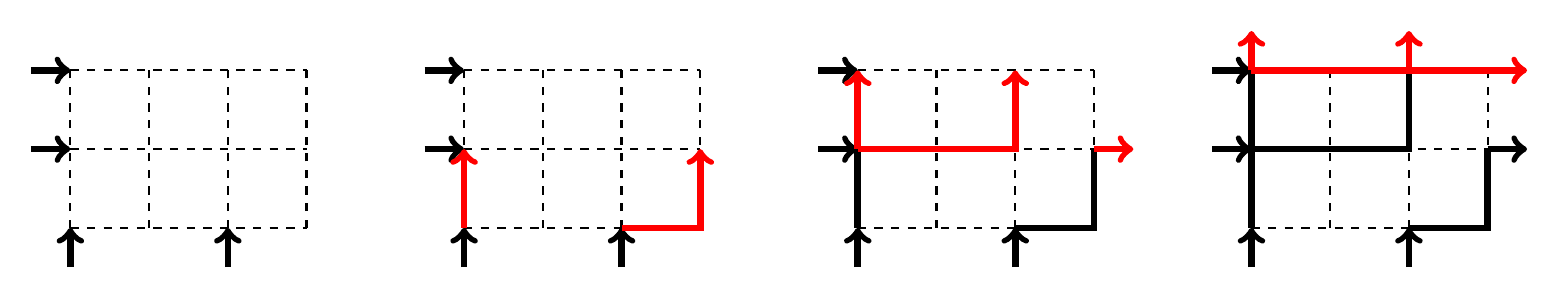
\begin{tikzpicture}
	[scale=1,thick]

\node at (0,2) {\phantom{$s$}};

	\foreach \ii in {0,...,3}
	{
	 \draw[dashed] (\ii,0)--++(0,2);
	}
	\foreach \jj in {0,...,2}
	{
	 \draw[dashed] (0,\jj)--++(3,0);
	}
	\draw[line width=2.4,->] (0,-.5)--++(0,.5);
	\draw[line width=2.4,->] (2,-.5)--++(0,.5);
	\draw[line width=2.4,->] (-.5,1)--++(.5,0);
	\draw[line width=2.4,->] (-.5,2)--++(.5,0);
	
%	\node[anchor=west] at (3.05,0) {$w_{u_y}$};
%	\node[anchor=west] at (3.05,1) {$w_{u_{y+1}}$};
%	\node[anchor=west] at (3.05,2) {$w_{u_{y+2}}$};

	
\begin{scope}[shift={(5,0)}]
	\foreach \ii in {0,...,3}
	{
	 \draw[dashed] (\ii,0)--++(0,2);
	}
	\foreach \jj in {0,...,2}
	{
	 \draw[dashed] (0,\jj)--++(3,0);
	}
	\draw[line width=2.4,->] (0,-.5)--++(0,.5);
	\draw[line width=2.4,->] (2,-.5)--++(0,.5);
	\draw[line width=2.4,->] (-.5,1)--++(.5,0);
	\draw[line width=2.4,->] (-.5,2)--++(.5,0);
	\draw[red, line width=2.4,->] (0,0)--++(0,1);
	\draw[red, line width=2.4,->] (2,0)--++(1,0)--++(0,1);
	
	% \node[anchor=west] at (3.05,0) {$w_{u_y}$};
%	\node[anchor=west] at (3.05,1) {$w_{u_{y+1}}$};
%	\node[anchor=west] at (3.05,2) {$w_{u_{y+2}}$};

\end{scope}

	
\begin{scope}[shift={(10,0)}]
	\foreach \ii in {0,...,3}
	{
	 \draw[dashed] (\ii,0)--++(0,2);
	}
	\foreach \jj in {0,...,2}
	{
	 \draw[dashed] (0,\jj)--++(3,0);
	}
	\draw[line width=2.4,->] (0,-.5)--++(0,.5);
	\draw[line width=2.4,->] (2,-.5)--++(0,.5);
	\draw[line width=2.4,->] (-.5,1)--++(.5,0);
	\draw[line width=2.4,->] (-.5,2)--++(.5,0);
	\draw[line width=2.4] (0,0)--++(0,1);
	\draw[line width=2.4] (2,0)--++(1,0)--++(0,1);
	
	\draw[red, line width=2.4,->] (0,1)--++(0,1);
	\draw[red, line width=2.4,->] (0,1)--++(2,0)--++(0,1);	
	\draw[red, line width=2.4,->] (3,1)--++(.5,0);		
	
%	\node[anchor=west] at (3.05,0) {$w_{u_y}$};
	% \node[anchor=west] at (3.05,.65) {$w_{u_{y+1}}$};
%	\node[anchor=west] at (3.05,2) {$w_{u_{y+2}}$};

\end{scope}

\begin{scope}[shift={(15,0)}]
	\foreach \ii in {0,...,3}
	{
	 \draw[dashed] (\ii,0)--++(0,2);
	}
	\foreach \jj in {0,...,2}
	{
	 \draw[dashed] (0,\jj)--++(3,0);
	}
	\draw[line width=2.4,->] (0,-.5)--++(0,.5);
	\draw[line width=2.4,->] (2,-.5)--++(0,.5);
	\draw[line width=2.4,->] (-.5,1)--++(.5,0);
	\draw[line width=2.4,->] (-.5,2)--++(.5,0);
	
	\draw[line width=2.4] (0,0)--++(0,1);
	\draw[line width=2.4] (2,0)--++(1,0)--++(0,1);
	
	\draw[line width=2.4] (0,1)--++(0,1);
	\draw[line width=2.4] (0,1)--++(2,0)--++(0,1);	
	\draw[line width=2.4,->] (3,1)--++(.5,0);
	
	\draw[red, line width=2.4,->] (0,2)--++(0,.5);
	\draw[red, line width=2.4,->] (0,2)--++(2,0)--++(0,.5);
	\draw[red, line width=2.4,->] (2,2)--++(1.5,0);
	
%	\node[anchor=west] at (3.05,0) {$w_{u_y}$};
%	\node[anchor=west] at (3.05,1) {$w_{u_{y+1}}$};
	% \node[anchor=west] at (3.05,1.65) {$w_{u_{y+2}}$};

\end{scope}
 
 \end{tikzpicture}
\end{document}

